%-------------------------------------------------------------------------------
\FloatBarrier\section{Dataset}
%-------------------------------------------------------------------------------
A documentation of the dataset is available in \cite{NLSY.2014}. Note that most of the graphs are based on the full NLSY and thus are not necessarily representative of the population.

\begin{figure}[htp]\centering
\caption{Observations over time}
\scalebox{0.35}{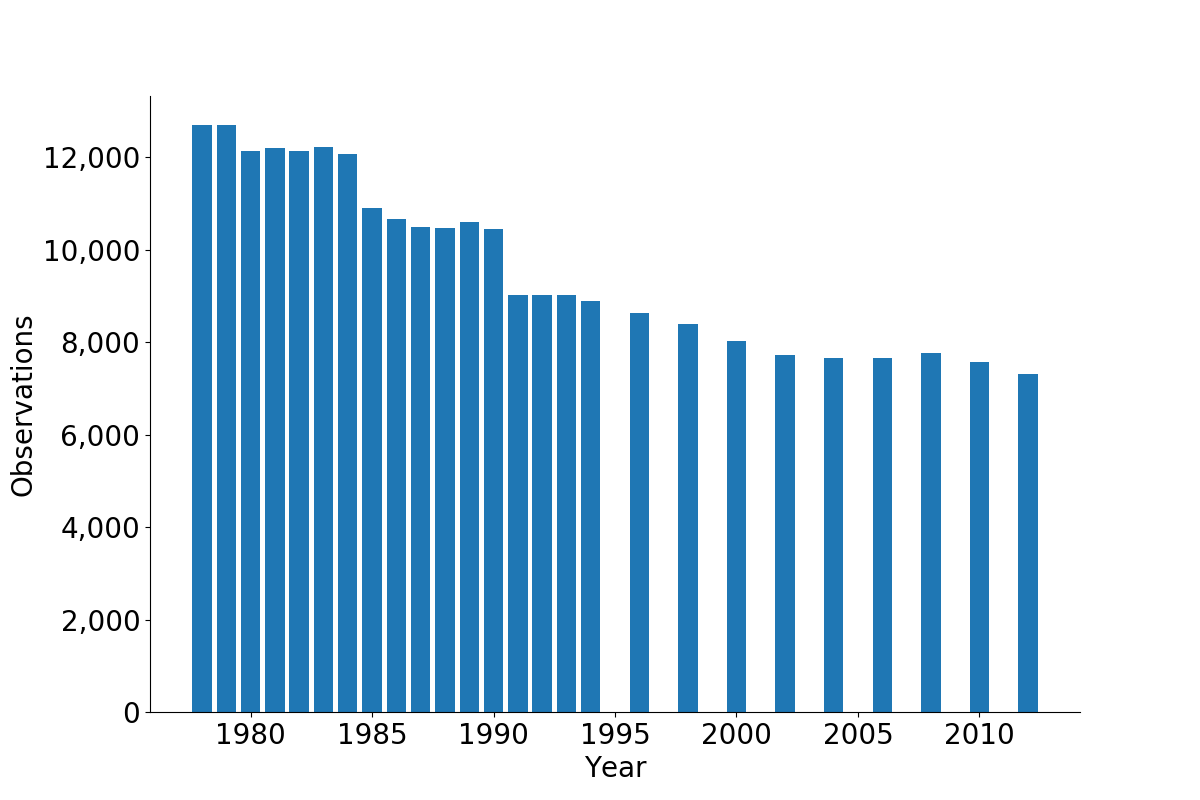
\includegraphics{fig-dataset-basic-observations}}
\end{figure}

\begin{figure}[htp]\centering
\caption{Samples in the NLSY}
\scalebox{0.35}{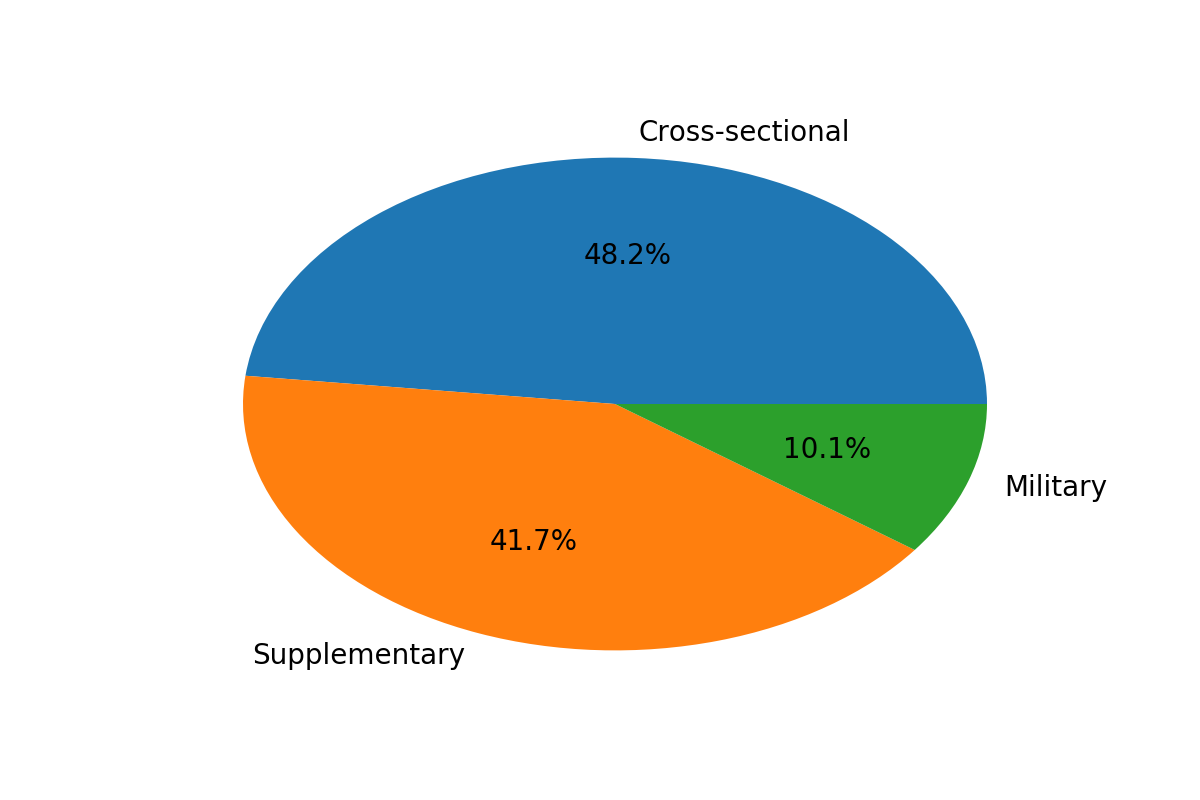
\includegraphics{fig-dataset-basic-samples}}
\end{figure}

\begin{figure}[htp]\centering
\caption{NLSY and gender}
\scalebox{0.35}{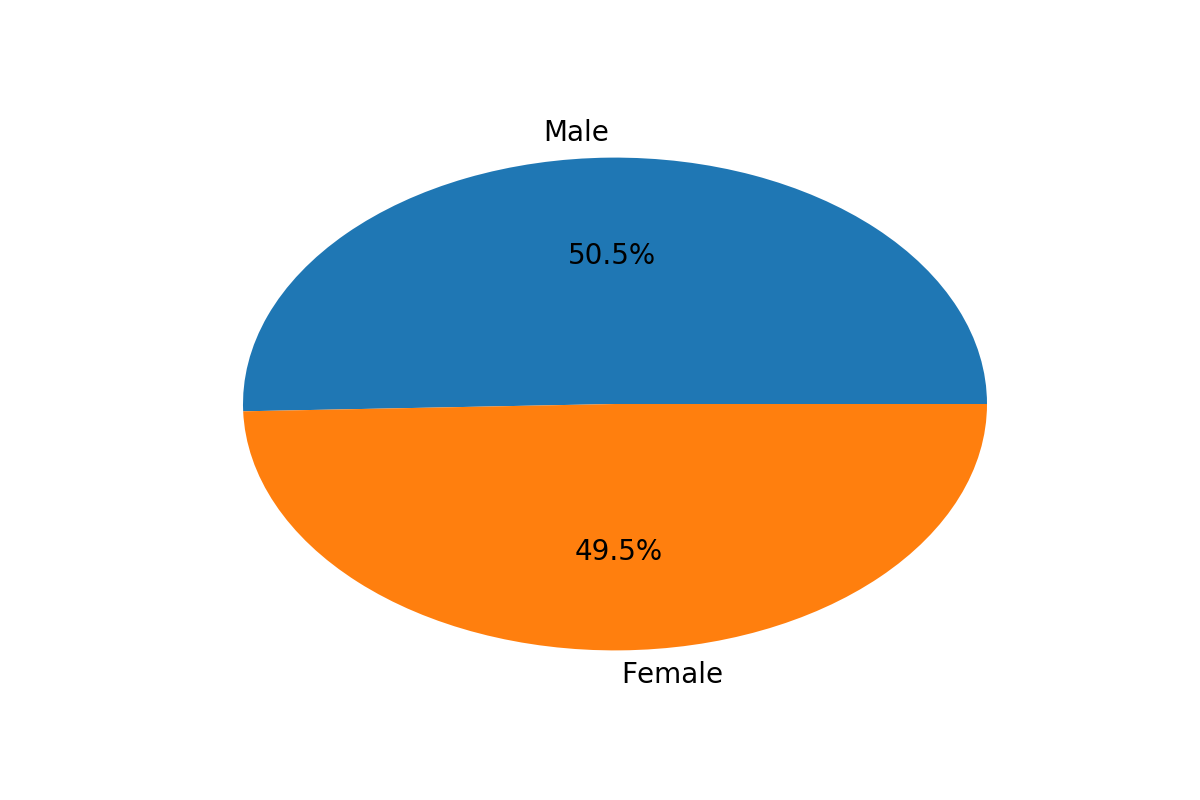
\includegraphics{fig-dataset-basic-gender}}
\end{figure}

Percentage of total income earned by income quartile (first quartile = 25\% of households with the lowest income). Read as households who are part of the 1st/2nd/3rd/4th quartile together earn x percentage of total income.

\begin{figure}[htp]\centering
\caption{NLSY and incomequartile}
\scalebox{0.35}{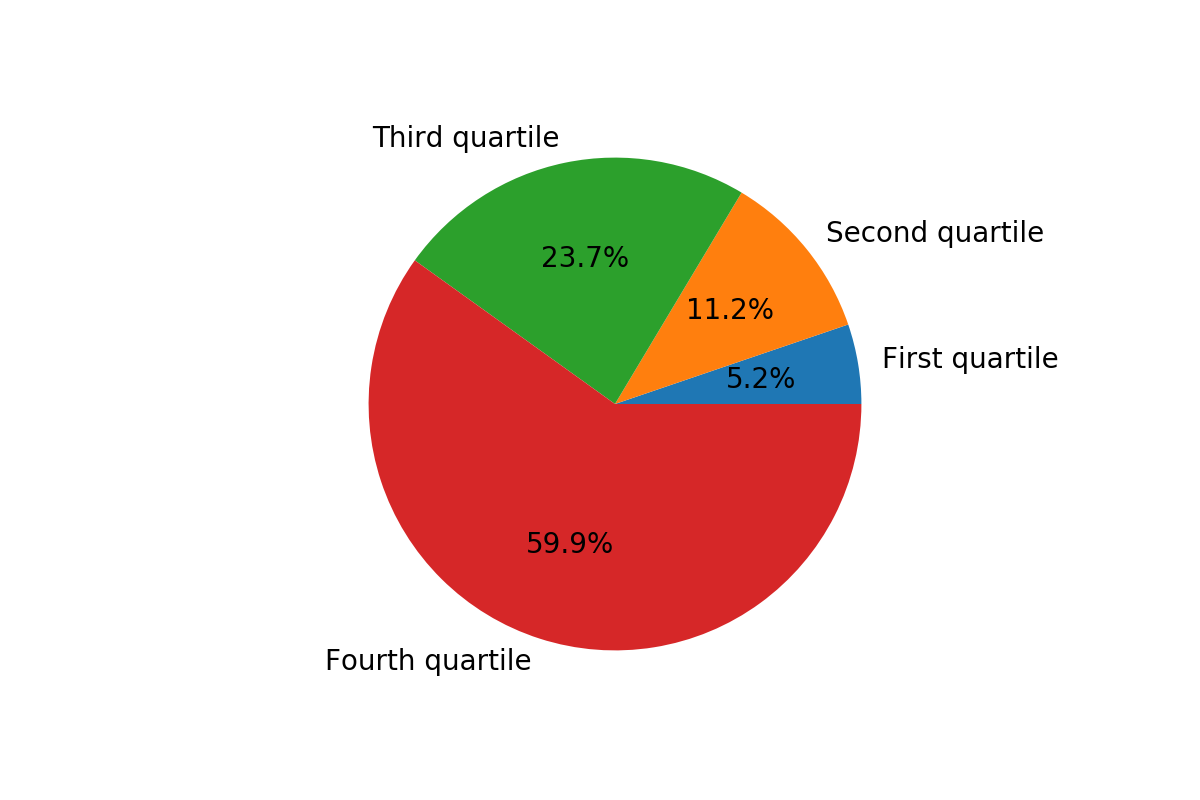
\includegraphics{fig-dataset-basic-income-quartile}}
\end{figure}

\begin{figure}[htp]\centering
\caption{NLSY and year of birth}
\scalebox{0.35}{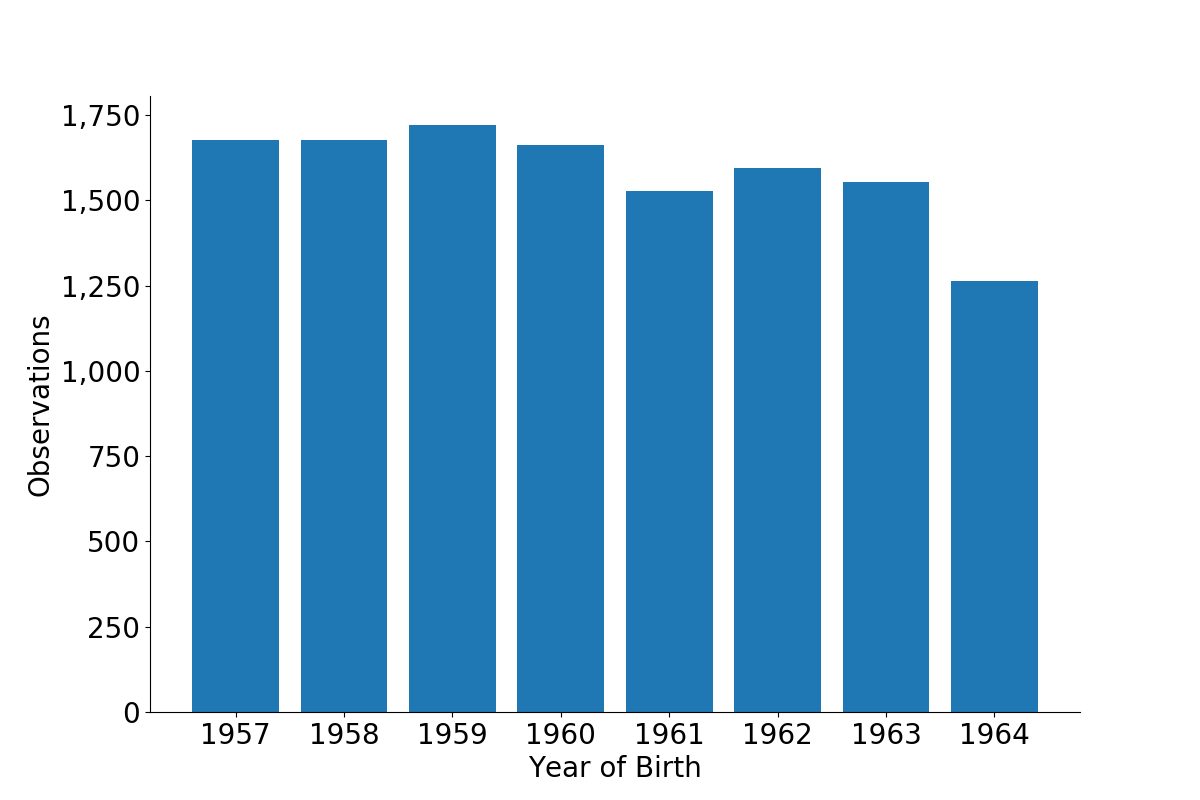
\includegraphics{fig-dataset-basic-birth}}
\end{figure}
